\documentclass[11pt]{article}
\title{Technical Report\\ COMP1100 Assignment 3}
\author{Jacob Bos\\ ANU u7469354}

\usepackage{graphicx}
\usepackage{amsmath}
\usepackage{amssymb}
\usepackage{array}
	\newcolumntype{L}{>{\centering\arraybackslash}m{15cm}}
\usepackage{float}
\usepackage{multicol}
\setlength{\columnsep}{1cm}
\usepackage{setspace}
\usepackage{xcolor}

\newenvironment{smallpmatrix}
  {\left(\begin{smallmatrix}}
  {\end{smallmatrix}\right)}
 \newenvironment{smol}
  {\left(\begin{smallmatrix}}
  {\end{smallmatrix}\right)}


\usepackage[margin=2cm]{geometry}
\addtolength{\textheight}{-0.5cm}
%~~~~~~~~~~~~~~~~~~~~~~~~~~~~~~~~~~~~~~~~~~~~~~~~~~~~~~~~~~~~~~~~~~~~~~~~~~~~~~~~~~~~~~~~~~~~~~~~~~~~
%~~~~~~~~~~~~~~~~~~~~~~~~~~~~~~~~~~~~~~~~~~~~~~~~~~~~~~~~~~~~~~~~~~~~~~~~~~~~~~~~~~~~~~~~~~~~~~~~~~~~
\begin{document}
\maketitle
\pagenumbering{roman}
\setstretch{1.5}
\begin{center}
  Lab: Tuesday 11am\\
  Tutor: Abhaas Goyal\\
  Word-count beyond cover page at $\leq 1500$ words
\end{center}
\tableofcontents
\newpage
\pagenumbering{arabic}
%~~~~~~~~~~~~~~~~~~~~~~~~~~~~~~~~~~~~~~~~~~~~~~~~~~~~~~~~~~~~~~~~~~~~~~~~~~~~~~~~~~~~~~~~~~~~~~~~~~~~
\section{Introduction} 
The program detailed herein is an implementation of a few AI's for solving the game Fanorona with complimentary unit tests.


%~~~~~~~~~~~~~~~~~~~~~~~~~~~~~~~~~~~~~~~~~~~~~~~~~~~~~~~~~~~~~~~~~~~~~~~~~~~~~~~~~~~~~~~~~~~~~~~~~~~~
\section{Documentation}%Explanation of code workings, functions and structure.
\subsection{Design Documentation and Technical Decisions}
% Describe what each relevant function does conceptually. (i.e. how does it get you closer to solving the problems outlined in this assignment spec?)
% How do these functions piece together to make the finished program? Why did you design and implement it this way?
% What major design choices did you make regarding the functions that you’ve written and the overall structure of your program?
\paragraph*{First capture move} is little more complex than the provided \verb|firstLegalMove|, it is "content" with taking the head of the list of possible capturing moves as provided by the function \verb|captures| else returning the first legal move. This was used to test the greedy AI, because a greedy should on average perform better than the first capture move which should beform slighly better than first legal move.

\paragraph{The Greedy AI} has a simple functionality. The main function \verb|greedy| cases on which player's turn it is given the provided gameState and chooses whether to maximize (for Player1) or minimize (for Player2) the heuristic value and calls \verb|greedyHelp| with the appropriate evaluator to output a pair containing the ideal move and its heuristic value. \verb|greedyHelp| recurses through a list of moves and their values and using an accumulator either minimizes or maximizes it. This list is a mapping of the list provided by \verb|legalMoves| to a list of pairs of moves of each move with the value of the move created by the function \verb|diffPieces| applied to the \verb|applyMove| of the move and initial state.

\paragraph{The first Minimax} uses two recursive tree structures, the first \verb|GameTree|, stores all the possible gamestate evolutions and is generated through an infinite recursion in \verb|gameTree| which takes a state, puts it into a node and then maps \verb|gameTree| to all its children states which are generated through a mapping of \verb|applyMove| to a list of \verb|legalMoves| which is then recursively purged of its \verb|[Maybe GameState]| type by \verb|purge| to become \verb|[GameState]|.

\subparagraph*{}The second tree structure, \verb|evalTree| is the same as \verb|GTree| except that it contains a value on each node corresponding to the best possible outcome (heuristic value) for the player who's state is at that node and is pruned to a given \textit{move depth}. The \verb|evalTree| is generated by recursively by \verb|pruneMinMax| which cases firstly on integer depth given to the function, if the depth is zero then it evaluated the heuristic value at that node and then terminates that branch. If not, it then cases on the state held in the node, if the state contains a \verb|GameOver| turn then it does as if the depth was zero, terminating the tree. If the state at a node contains \verb|Turn Player1| then it assigns the maximum of the values in its child \verb|EvalTree| nodes else if the turn is the \verb|Player2|, the minimizing player, it assigns the minimum value of its child nodes to the given node. This results in the best possible outcome for the player in the initial state ending up in the head node.

\subparagraph*{}The heuristic value used is the difference in number of pieces between \verb|Player1| and \verb|Player2| and is calculated by \verb|heuristicVal| which takes the pair output of the provided \verb|countPieces| function and then takes the difference in the number of pieces.

\subparagraph*{}To then retrieve the best move we note that the best move is at the same depth in the \verb|legalMoves| list as best value stored in the head node is in the list of child \verb|evalTree| nodes. This is because the list of children nodes is produced by a mapping on the \verb|legalMoves| list. Consequently to find the best move we extract the value from the head of the output of \verb|pruneMinMax| using \verb|getVal| and then find it's depth recursively in the list provided by mapping \verb|getVal| to the child nodes at depth 1 using \verb|findDepth|. Consequently the function \verb|getMove| uses the (!!) operator to extract the best move at its expected depth in the \verb|legalMoves| list.

\paragraph*{The second Minimax} Is identical to the first except that the heuristic function assigns win or loss gamestates with heuristic values far more extreme their typical values. This was an experiment to see wether this would allow the AI to prioritize winning moves during the endgame and it improves results by a little bit.

\newpage
\subsection{Program Design / Structure}
The function dependencies of the greedy AI and both MiniMax AI's is featured below:
\begin{center}
  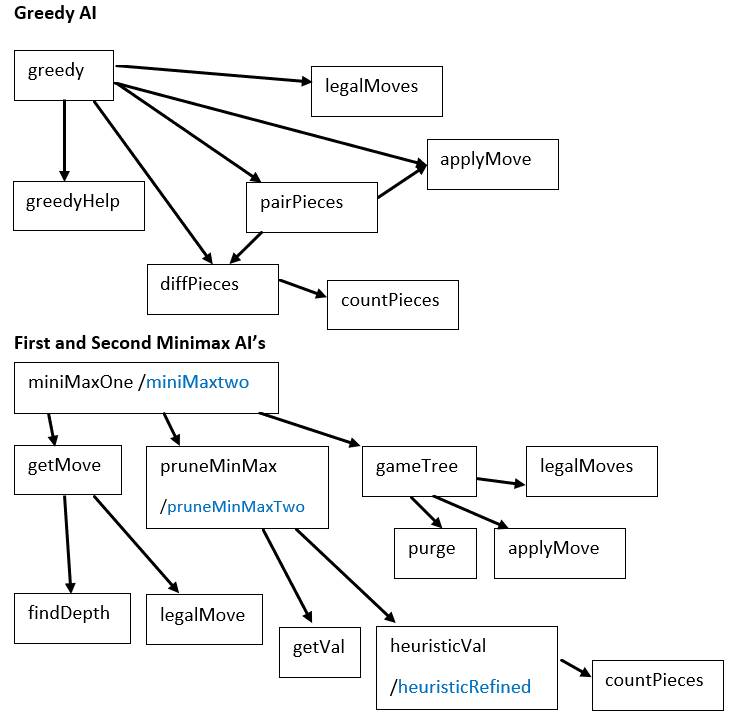
\includegraphics[width=0.85\textwidth]{functDep.png}
\end{center}

\paragraph{The Greedy AI's} structure somewhat convoluted and could be made simpler. As it stands it does a lot of unnecessary work with Maybe types which could be eliminated with the strategies used in the minimax AIs however was developed first. As a result of the extra case statements required to work with the maybe types it was necessary to break the AI into a number of helpers to improve style and readability.

\paragraph{The MiniMax AI's} share the same structure and the majority of their functions. Both are called by a top end function that inputs the initial states and calls a function that gets the move based on the result of the pruner function's evaluation tree. It was chosen to move \verb|getVal| to a helper function to reduce the things in the \verb|where| clause of the pruner to just static evaluations and not called functions.

 \subsection{Assumptions}%Describe assumptions you have made about how a user might use the program and how this has influenced your design decisions.
The primary assumption made is that the ordering of the \verb|legalMoves| list is the same as the ordering of their corresponding values in the \verb|depth=1| level of the \verb|EvalTree|. This assumption was made because despite \verb|purge| removing all nothings from list of subsequent states there would be no nothings because they only result from an illegal move being fed to \verb|applyMove| which is impossible when the \verb|legalMoves| list is used. Thus the values in the first child nodes are essentially the result of repeated mappings onto the \verb|legalMoves| list and so order is preserved. A second assumption made was the the \verb|legalMoves| list would never be empty because this would be prohibited by the game ending at that point. Consequently it was acceptable for \verb|findDepth| to return an error for an empty list.

%~~~~~~~~~~~~~~~~~~~~~~~~~~~~~~~~~~~~~~~~~~~~~~~~~~~~~~~~~~~~~~~~~~~~~~~~~~~~~~~~~~~~~~~~~~~~~~~~~~~~
\newpage
\section{Testing}%How did I test the program focus on methodology and testing groups
%How did you test individual functions?
%Be specific about this - the tutors know that you have tested your program, but they want to know how.
%Describe the tests that prove individual functions on their own behave as expected (i.e. testing a function with different inputs and doing a calculation by hand to check that the outputs are correct).
%How did you test the entire program? What tests did you perform to show that the program behaves as expected in all (even unusual) cases?
\paragraph{Unit tests} aimed to cover as many possible cases on as many functions as possible. Unfortunately, many of the functions deal with complex datatypes which makes it difficult to write typical arguments. Consequently many tests used \verb|initialState| and checked the length of the argument and desired output lists.

\subparagraph{The Greedy AI} has two associated test groups. \verb|pairPieces| was tested by checking that the list of pairs of legal moves and their associated heuristic value is the same length as the list of \verb|legalMoves|. The passing of this test is able to support the assumption that the function is correct. Secondly, \verb|diffPieces| is tested against two cases which were possible to write. It tested that the function returned \verb|Nothing| for the same argument and returned \verb|Just 0| for an input of just the initial state.

\subparagraph{The MiniMax AI} has four associated test groups. Firstly \verb|purge| has four test cases. They were made easier to write because \verb|purge| is polymorphic and so a simpler input type of \verb|Int| was used. \verb|purge| is then tested against a case of the empty list, all \verb|Nothing|s, all \verb|Just x|'s and a mix of \verb|Nothing|s and \verb|Just|s. Passing these tests implied that the function was correct. Similarly, since \verb|findDepth| is polymorphic it was easier to write test cases. It was not tested against the empty list since that was supposed to return an error but is was tested against cases where the element occurred once or twice in the list where its supposed to take the first. The passing of this indicated correctness. Thirdly, \verb|getVal| was tested against one test case, indicating it's ability to correctly retrieve the value from a node. Lastly \verb|heuristicVal| was tested with the initial state as an argument to ensure that the output is zero as would be expected. Unfortunately it was difficult to test it against any other inputs as other arguments are difficult to write.

\paragraph{Performance tests} were done by playing my AI's against themselves and also against the course AI's in the tournament.

\subparagraph{The Greedy AI} was firstly tested against both the first legal move AI and the first capture move AI. The correctness of the Greedy AI was confirmed by it beating both as it should statistically behave better than both. Whilst a faulty Greedy may be able to beat FLM by chance it is less likely to beat an FCM by chance especially if it was accidentally minimizing when it was supposed to maximize or vices-versa. Since the Greedy AI was also able to consistently beat me as a human I considered that it had a high likelihood pof being correct.

\subparagraph{The MiniMax AI's} were tested against both my greedy AI and the Course AIs, my MiniMax consistently outperformed my greedy and all of the course greedy AIs except for third where playing first results in a draw. My AI majority draws against the course Minimaxes and Alpha-beta pruners further indicating correctness. It would be expected with such a simple heuristic that another minimax or minimax-alpha/beta AI with a better heuristic would slightly outperform. 

%~~~~~~~~~~~~~~~~~~~~~~~~~~~~~~~~~~~~~~~~~~~~~~~~~~~~~~~~~~~~~~~~~~~~~~~~~~~~~~~~~~~~~~~~~~~~~~~~~~



\newpage
\section{Reflection}
%Discuss the reasoning behind your decisions, rather than what the decisions were. You can reflect on not only the decisions you made, but the process through which you developed the final program:
  %What would you have done differently if you were to do it again
    %What changes to the design and structure you would make if you wrote the program again from scratch?
  \subsection{Design Choices}
  For the greedy AI and the first minimax it was decided to use just the difference of pieces as the heuristic function as it was easily implemented by using the \verb|countPieces| function provided in \verb|Fanorona.hs|. This was done to allow myself greater time to design and understand the actual algorithms. However the second Minimax used the update describes in an attempt to prioritize winning moves in endgame. It was chosen that the greedy AI should pair moves with their associated value to allow for an accumulator recursion to find the move with the best outcome. In contrast the minimax AI's did not store moves in the structure relying on the discussed assumption about list lengths. This was done in order to simplify the structures and functions as much as possible in an attempt to improve style and speed for example by being able to use pre-optimized functions like \verb|maximize| and avoid convoluted datatype that require using functions like \verb|fmap|. The minimax pruners were designed to make as good use of laziness as possible. This allowed a node to be assigned the minimum of maximum value of its children before the children were evaluated. This meant that it was only necessary to navigate down the tree.

  \subsection{Reflection}
  Upon reflection I would have designed my functions to take a heuristic function as an input so as to not need to rewrite the pruner function but rather to take a heuristic function as an argument. Further I would have removed the states from the nodes of the \verb|EvalTree| to simplify the structure even more.



%~~~~~~~~~~~~~~~~~~~~~~~~~~~~~~~~~~~~~~~~~~~~~~~~~~~~~~~~~~~~~~~~~~~~~ ~~~~~~~~~~~~~~~~~~~~~~~~~~~~~~~


%~~~~~~~~~~~~~~~~~~~~~~~~~~~~~~~~~~~~~~~~~~~~~~~~~~~~~~~~~~~~~~~~~~~~~~~~~~~~~~~~~~~~~~~~~~~~~~~~~~~~
\end{document}
